% SVN info for this file
\svnidlong
{$HeadURL$}
{$LastChangedDate$}
{$LastChangedRevision$}
{$LastChangedBy$}

\chapter{The User Acceptance Testing Framework}
\labelChapter{Chapter_2}

\begin{introduction}
  This chapter will guide through the steps of creating and running a BDD scenario for BMI via the User Acceptance Framework.
\end{introduction}

\section{The User Acceptance Testing Architecture}

You will need to be provided a compressed (\emph{tar.gz}) file of the acceptance tests.  After you uncompress it via the \code{"tar -xzvf acceptance-tests.tar.gz"} you will see the following files and folders in the root directory:


\begin{figure}[!h] % Example of including images
\vspace{10mm}
\label{fig:uat-root-dir}
\begin{center}
%\includegraphics[width=0.5\linewidth]{#1}
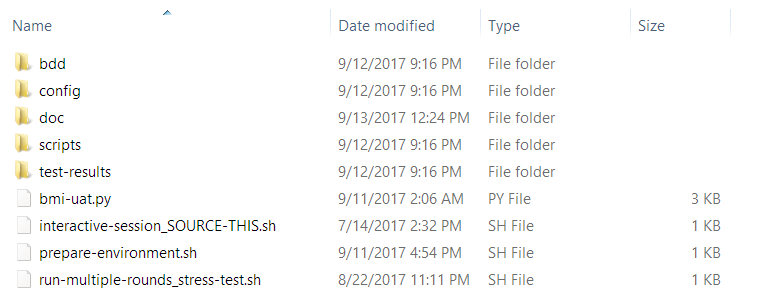
\includegraphics[scale=0.8]{figures/uat-root-dir.png}
\end{center}
\caption{Root directory of the User Acceptance Testing framework}
%\label{fig:example_figure}
\end{figure}

%\pagebreak
Below are descriptions of the critical folders and files required for configuring and for running the tests: \\

\begin{itemize}
\item[\index{config directory}\code{config }$\blacktriangleright$\hspace{-12mm}] \hspace{10mm}\emph{Contains the testing configurations for different environments (i.e. PRB, NEU, etc).}
\item[\index{doc directory}\code{doc }$\blacktriangleright$\hspace{-12mm}] \hspace{10mm}\emph{Contains this manual.}
\item[\index{scripts directory}\code{scripts }$\blacktriangleright$\hspace{-12mm}] \hspace{10mm}\emph{Contains the configuration scripts that are run for different stages during testing.}

\item[\index{prepare-environment.sh script}\code{prepare-environment.sh }$\blacktriangleright$\hspace{-12mm}] \hspace{10mm}\emph{Configurations to run for different OS environments before testing, which can be \\ \text{}\hspace{9mm} used to create cleanup scripts.}

\item[\index{bmi-uat.py script}\code{bmi-uat.py }$\blacktriangleright$\hspace{-12mm}] \hspace{10mm}\emph{The command-line interface (CLI) for listing and running the tests.}


\item[\index{test-results}\code{test-results }$\blacktriangleright$\hspace{-12mm}] \hspace{10mm}\emph{Provides test results in case one performs randomized tests for multiple rounds.} \\
\end{itemize}

The \code{interactive-session\_SOURCE-THIS.sh} script is used if you want to drop into an interactive session into the environment of a particular test after is completed in order to inspect or rollback changes. \\

Next you will learn about the \code{config} directory regarding how to use or create new testing environments.

\subsection{Configuring a Testing Environment}

If you look at the \code{config} directory you will see something that looks similar to this:

\begin{figure}[!h] % Example of including images
\vspace{10mm}
\begin{center}
%\includegraphics[width=0.5\linewidth]{#1}
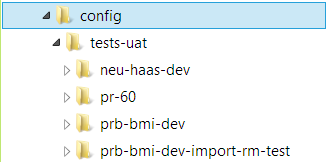
\includegraphics[scale=1]{figures/uat-config-dir.png}
\end{center}
\caption{\code{Config} directory of the User Acceptance Testing framework}
%\label{fig:example_figure}
\label{fig:uat-root-dir}
\end{figure}

It is best to copy a previous directory of interest if you would like to perform the minimal changes to a test.  There are two types of test directories: \\

\begin{itemize}
\item[\index{\code{Pull-Request Test}}\code{Pull-Request Test }$\blacktriangleright$\hspace{-12mm}] \hspace{10mm}\emph{Performs tests on a specific pull-request (i.e. \emph{pr-60}).  These are usually performed \underline{in preparation for running a deployment test}.} \\

\item[\index{\code{Repository Test}}\code{Repository Test }$\blacktriangleright$\hspace{-12mm}] \hspace{10mm}\emph{Performs tests on a whole repository (i.e. \emph{neu-haas-dev}).  These would be performed to ensure a \underline{release is ready for deployment}.} \\

\end{itemize}

Next we will look at how a test configuration is structured.

\subsection{Structure of Test Directory}

If you look at any of the test directories they all look as follows:

\begin{figure}[!h] % Example of including images
\vspace{10mm}
\begin{center}
%\includegraphics[width=0.5\linewidth]{#1}
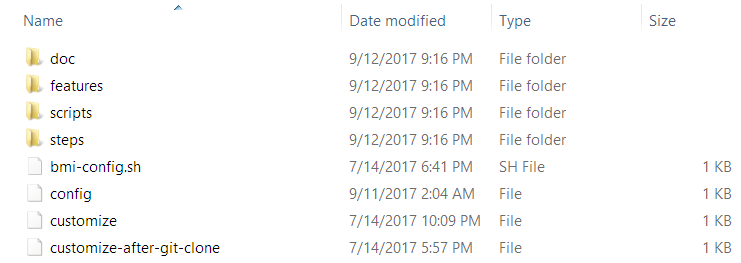
\includegraphics[scale=0.8]{figures/uat-test-dir.png}
\end{center}
\caption{The test directory structure}
%\label{fig:example_figure}
\label{fig:uat-root-dir}
\end{figure}

To keep the configurations simple and practical, it is important to know about the following four components: \\

\begin{itemize}


\item[\index{config directory}\code{config }$\blacktriangleright$\hspace{-12mm}] \hspace{10mm}\emph{This file configures the BMI UAT test for the environment, and is the most \underline{important}\\ \text{}\hspace{9mm} file.} \\

\item[\index{\code{bmi-config.sh} script}\code{bmi-config.sh }$\blacktriangleright$\hspace{-12mm}] \hspace{10mm}\emph{This is the second most important file, and is used to configure the BMI pre-test\\ \text{}\hspace{9mm} deployment directories.} \\

\item[\index{BDD features}\code{features }$\blacktriangleright$\hspace{-12mm}] \hspace{10mm}\emph{These contain the live documents that can be changed with the exception of the\\ \text{}\hspace{9mm} \emph{template} file.  Additional scenario files to test for can be added if preferred.} \\

\item[\index{BDD steps}\code{steps }$\blacktriangleright$\hspace{-12mm}] \hspace{10mm}\emph{Contains the functions that map to the given BDD definition in the \emph{feature} files\\ \text{}\hspace{9mm} that build up the scenarios.} \\

\end{itemize}

\subsection{The \code{config} file}

The \code{config} file is usually the only file one will usually configure the most of the time, and it was created to ensure minimal changes are necessary for test-preparation.  The structure of the file is shown in Figure \ref{fig:uat-config-file}, and is composed of the following three main sections: \\ % has the following structure:

\begin{itemize}
\item[\index{\code{BMI\_RELEASE\_NAME}}\code{BMI\_RELEASE\_NAME }$\blacktriangleright$\hspace{-12mm}] \hspace{10mm}\emph{This will denote the name of the directory for the scenario that is being tested, \\ \text{}\hspace{9mm} underneath which the tests will be installed, configured and run.} \\

\pagebreak

\item[\index{\code{E2E Test Configs}}\code{E2E Test Configs }$\blacktriangleright$\hspace{-12mm}] \hspace{10mm}\emph{The middle section contains the End-To-End configuration information that are\\ \text{}\hspace{9mm} pertinent to the environment being tested (i.e. HIL project names, names of BMI\\ \text{}\hspace{9mm} images to create, etc).} \\

\item[\index{\code{BMI and HIL Configurations}}\code{BMI and HIL Configs }$\blacktriangleright$\hspace{-12mm}] \hspace{10mm}\emph{These contain the HIL and BMI local configurations in order for the tests to run.} 

\end{itemize}

\begin{figure}[!h] % Example of including images
\vspace{10mm}
%\label{fig:uat-config-file}
\begin{center}
%\includegraphics[width=0.5\linewidth]{#1}
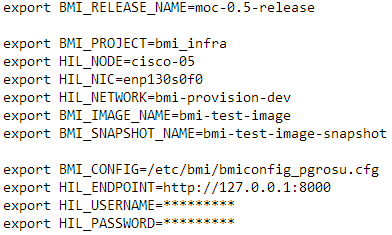
\includegraphics[scale=1]{figures/uat-config-file.png}
\end{center}
\caption{The test configuration file structure}
\label{fig:uat-config-file}
\end{figure}

An example of the \code{bmi-config.sh} file is shown in Figure \ref{fig:uat-config-file}, which provides the configurations of where the BMI instance will be installed (\code{BMI\_INSTANCE\_DIR}), and the location of the User Acceptance Tests directory (\code{ACCEPTANCE\_TESTS\_SRC\_DIR}).


\begin{figure}[!h] % Example of including images
\vspace{10mm}
\begin{center}
%\includegraphics[width=0.5\linewidth]{#1}
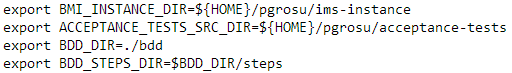
\includegraphics[scale=1]{figures/uat-bmi-config.png}
\end{center}
\caption{An example of a \code{bmi-config.sh} file}
%\label{fig:example_figure}
\label{fig:uat-bmi-config}
\end{figure}



\section{Preparing The Environment \\} 

Sometimes the operating environment requires extra functionality -- such as Python or Git availability -- to be available before running a test.  These configurations can be placed as Bash scripts under the \code{scripts\textbackslash prepare-environments} directory, as shown in Figure \ref{fig:uat-prepare-environment}.

\pagebreak

\begin{figure}[!h] % Example of including images
\vspace{10mm}
\begin{center}
%\includegraphics[width=0.5\linewidth]{#1}
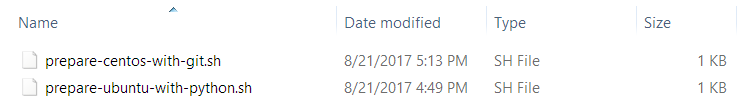
\includegraphics[scale=0.9]{figures/uat-prepare-environment.png}
\end{center}
\caption{An example of the \code{prepare-environments} directory}
%\label{fig:example_figure}
\label{fig:uat-prepare-environment}
\end{figure}

To list all configurations, type under the main \code{acceptance-tests} directory \code{./prepare-environment.sh}, as shown in Figure \ref{fig:uat-prepare-environment-list}.


\begin{figure}[!h] % Example of including images
\vspace{10mm}
\begin{center}
%\includegraphics[width=0.5\linewidth]{#1}
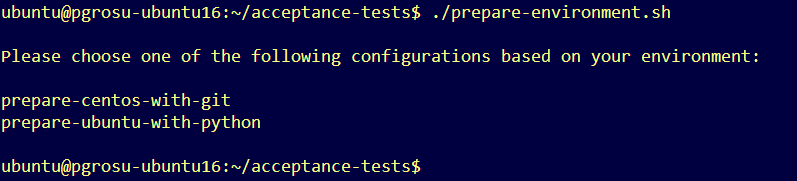
\includegraphics[scale=0.9]{figures/uat-prepare-environment-list.png}
\end{center}
\caption{Listing the \code{prepare-environments} configurations}
%\label{fig:example_figure}
\label{fig:uat-prepare-environment-list}
\end{figure}

To run a configuration just use the following format to run the appropriate configuration for your environment: \\

\begin{center}
\code{./prepare-environment.sh \emph{CONFIGURATION}}
\end{center}

Now you are ready to run a test configuration.

\section{Performing the Acceptance Tests \\} 

\index{running User Acceptance Tests}The performance tests can be initiated via the following steps: \\

\begin{enumerate}

\item  To list the testable BMI service configurations, type the following command: \\

\code{\text{}\hspace{6mm}    ./bmi-uat.py ls } \\

%\pagebreak

You should see something like the following:

\code{
\text{}\hspace{12mm}   \\
\text{}\hspace{6mm}   The available configurations are: \\
\text{}\hspace{12mm}   \\
\text{}\hspace{12mm}   neu-haas-dev \\
}

\item To run the standard end-to-end configuration, type the following command: \\

\code{\text{}\hspace{6mm}     ./bmi-uat.py -{}-run BMI\_SERVICE\_CONFIGURATION} \\

  Example: \\

\code{\text{}\hspace{6mm}     ./bmi-uat.py -{}-run neu-haas-dev} \\

%\pagebreak

At the end you if the tests passed successfully, you should see the following output: \\

\begin{figure}[!h] % Example of including images
%\label{fig:ceph-imported-cloned-image}
\begin{center}
%\includegraphics[width=0.5\linewidth]{#1}
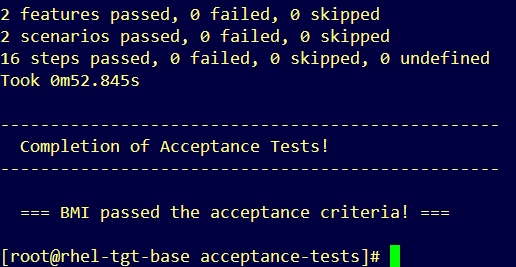
\includegraphics[scale=0.7]{figures/bdd-bmi-passed-tests.png}
\end{center}
\caption{The BMI completed successfully the end-to-end scenario}
%\label{fig:example_figure}
\label{fig:bdd-bmi-example-successful}
\end{figure}

\item To run the tests with randomized parameters, type the following where the value indicates the number of times to run the test: \\

\code{\text{}\hspace{6mm}     ./bmi-uat.py -{}-run neu-haas-dev -{}-randomize 3 } \\

\item To check if the tests passed or failed, type the following: \\

\code{\text{}\hspace{6mm}       ./bmi-uat.py check } \\

  You should see the following: \\
 
\code{\text{}\hspace{6mm}         All tests passed! } \\

  This command checks the \code{test-results} directory for any subdirectory containing \code{FAIL} in its name. \\
 
\item To cleanup all previous results, type the following: \\

\code{\text{}\hspace{6mm}       ./bmi-uat.py clean } \\

\end{enumerate}

You will notice that when running a test, there are many additional sanity-checks that are being made to ensure each test not only completes properly, but also provides sufficient detail in case of failure, as shown by the following figure:

\begin{figure}[!h] % Example of including images
\vspace{10mm}
\begin{center}
%\includegraphics[width=0.5\linewidth]{#1}
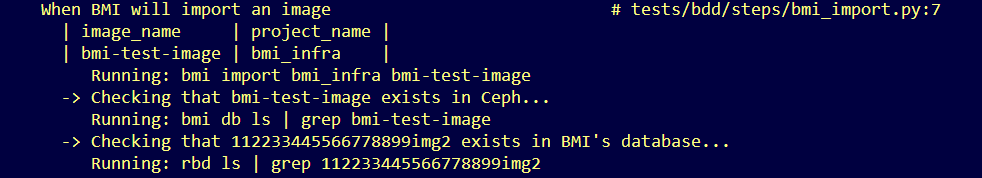
\includegraphics[scale=0.7]{figures/uat-test-check.png}
\end{center}
\caption{Sanity-checks for the \code{BMI import} step}
%\label{fig:example_figure}
\label{fig:uat-prepare-environment-list}
\end{figure}



\subsection{Entering an Interactive Session}

After the test has completed -- either successfully or not -- one can enter an \index{interactive session}interactive session to inspect the state of the test, where BMI commands can be executed interactively.  This is performed from the \code{acceptance-tests} directory by typing the following command -- make sure to not forget the period (.) at the before the script-name:

\begin{center}
\code{. interactive-session\_SOURCE-THIS.sh}
\end{center}

If the test was based on a pull-request, please add \code{--pr} as follows:

\begin{center}
\code{. interactive-session\_SOURCE-THIS.sh --pr}
\end{center}

You should see something as follows, showing that one is an virtual environment:

\begin{center}
\code{(.bmi\_venv) ubuntu@pgrosu-ubuntu16:$\sim$/ims-instance/ims\$}
\end{center}

To exit the interactive session, just type the following command -- from within the session:

\begin{center}
\code{. return-back-to-acceptance-dir\_SOURCE-THIS.sh}
\end{center}

By following the above steps you can now test your own customizations of BMI any services.
